\documentclass[a4paper, 12pt]{article}
\usepackage[utf8]{inputenc}
\usepackage[top=2cm, bottom=2cm, left=3cm, right=3cm]{geometry}
\usepackage{amsfonts, amsmath, amssymb}
\usepackage{graphicx}
\usepackage{amsthm}
\usepackage{amsmath}
\usepackage{amsfonts}
\usepackage{amssymb}
\usepackage{ifthen}
\usepackage{fancyhdr}
\usepackage{systeme}
\usepackage{amsthm}
\usepackage{geometry}
\usepackage[brazil]{babel}
\usepackage{indentfirst}
\usepackage{booktabs}
\usepackage{hyperref}
\usepackage[utf8]{inputenc}
\usepackage{IEEEtrantools}
\usepackage{changepage}
\usepackage{float}
\usepackage{listings}
\usepackage{color}
\usepackage[T1]{fontenc}
\usepackage{xfrac}
\definecolor{dkgreen}{rgb}{0,0.6,0}
\definecolor{gray}{rgb}{0.5,0.5,0.5}
\definecolor{mauve}{rgb}{0.58,0,0.82}
\lstset{
    language=Python,
    literate=
        {á}{{\'a}}1
        {à}{{\`a}}1
        {ã}{{\~a}}1
        {é}{{\'e}}1
        {ê}{{\^e}}1
        {í}{{\'i}}1
        {ó}{{\'o}}1
        {õ}{{\~o}}1
        {ú}{{\'u}}1
        {ü}{{\"u}}1
        {ç}{{\c{c}}}1,
    basicstyle=\ttfamily\tiny\footnotesize,
    numbers=left,
    numberstyle=\tiny\color{gray},
    stepnumber=2,
    numbersep=5pt,
    backgroundcolor=\color{white},
    showspaces=false,
    showstringspaces=false,
    showtabs=false,
    frame=single,
    rulecolor=\color{black},
    tabsize=1,
    captionpos=b,
    breaklines=true,
    breakatwhitespace=false,
    title=\lstname,
    keywordstyle=\color{blue},
    commentstyle=\color{dkgreen},
    stringstyle=\color{mauve},
}
\title{Primeiro Trabalho Computacional}
\author{
    Victor Rodrigues de Carvalho Leal Monteiro\
    N°USP: 11809902 \\
    \\
    {\textbf{Professor: Prof. Dr. Luis Carlos de Castro Santos}}}
\date{IME-USP 2025}
\begin{document}
    \maketitle

%==========================================================

    \section*{Dedução de \( g(x,t) \)}

    Dada a EDP parabólica e a solução manufaturada proposta:
    \[
        u_t = u_{xx} + g(x,t), \quad 0 < x < 1
    \]
    \[
        u(x,t) = e^{-t} \sin\left( \frac{\pi}{2} x \right) \cos\left( \frac{\pi}{2} x \right)
    \]

    Usando a identidade trigonométrica \(\sin a \cos a = \frac{1}{2}\sin(2a)\), obtém-se:
    \[
        u(x,t) = \frac{1}{2} e^{-t} \sin(\pi x)
    \]

    Derivando em relação a \(t\):
    \[
        u_t = -\frac{1}{2} e^{-t} \sin(\pi x)
    \]

    Derivando duas vezes em relação a \(x\):
    \[
        u_{xx} = -\frac{\pi^2}{2} e^{-t} \sin(\pi x)
    \]

    Substituindo na EDP e isolando \(g(x,t)\):
    \[
        -\frac{1}{2} e^{-t} \sin(\pi x) = -\frac{\pi^2}{2} e^{-t} \sin(\pi x) + g(x,t)
    \]
    \[
        \boxed{g(x,t) = \frac{\pi^2 - 1}{2} e^{-t} \sin(\pi x)}
    \]

    Dado o problema de condições de contorno de Dirichlet resultante, aplicaram-se ambos os métodos Forward Difference e Crank-Nicolson em Python, cujos resultados serão exibidos abaixo.

%==========================================================
    \pagebreak


    \section{Resultados Numéricos}

    \subsection{Tabela de Convergência}

    \begin{table}[H]
        \centering
        \caption{Resultados do método Forward Difference para diferentes refinamentos de malha}
        \label{tab:convergencia}
        \begin{tabular}{cccccc}
            \toprule
            $h$    & $k$      & $N_t$ & $k/h^2$ & Erro $L^2$            & Taxa de Convergência \\
            \midrule
            0.1000 & 0.004926 & 203   & 0.4926  & $1.37 \times 10^{-3}$ & --                   \\
            0.0500 & 0.001238 & 808   & 0.4952  & $3.42 \times 10^{-4}$ & 2.00                 \\
            0.0250 & 0.000310 & 3226  & 0.4960  & $8.51 \times 10^{-5}$ & 2.01                 \\
            \bottomrule
        \end{tabular}
    \end{table}


    \section{Análise Gráfica}

    \begin{figure}[H]
        \centering
        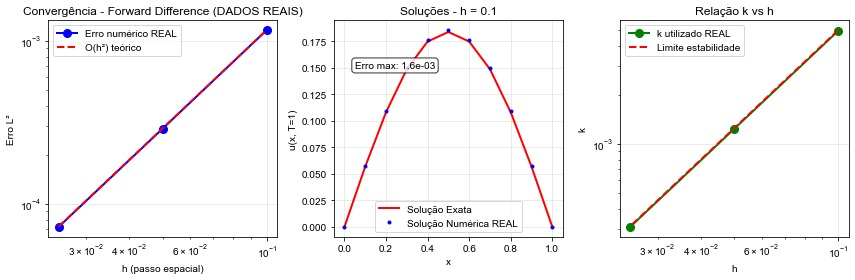
\includegraphics[width=\textwidth]{imgs/graficos_dados_reais}
        \caption{Resultados das simulações numéricas: (a) Convergência do erro, (b) Comparação entre soluções numérica e analítica, (c) Relação entre os passos espacial e temporal}
        \label{fig:resultados}
    \end{figure}

    \subsection{Análise do Gráfico de Convergência}

    O gráfico de convergência demonstra o comportamento do erro na norma $L^2$ em função do refinamento da malha espacial $h$. Observa-se que:

    \begin{itemize}
        \item O erro decresce quadraticamente com $h$, conforme esperado teoricamente
        \item A taxa de convergência calculada aproxima-se de 2, validando a implementação do método
        \item A linha tracejada vermelha representa a convergência teórica $O(h^2)$
        \item Os pontos azuis representam os erros reais obtidos nas simulações
    \end{itemize}

    A relação observada confirma que o método Forward Difference possui ordem de convergência $O(h^2)$ quando o passo temporal $k$ é escolhido proporcional a $h^2$.

    \subsection{Análise da Comparação de Soluções}

    O gráfico de comparação mostra a solução numérica e analítica no tempo final $t = 1$ para $h = 0.1$. Nota-se:

    \begin{itemize}
        \item Boa concordância entre as soluções numérica e analítica
        \item Pequenas discrepâncias devido aos erros de truncamento do método
        \item O erro máximo local é indicado no gráfico, proporcionando uma medida da precisão pontual
        \item As condições de contorno são satisfeitas corretamente ($u(0,t) = u(1,t) = 0$)
    \end{itemize}

    A forma senoidal da solução é preservada pelo método numérico, demonstrando sua adequação para este tipo de problema.

    \subsection{Análise da Relação k vs h}

    O gráfico da relação entre os passos temporal e espacial ilustra:

    \begin{itemize}
        \item Os valores de $k$ utilizados nas simulações (pontos verdes)
        \item O limite teórico de estabilidade $k = \frac{1}{2}h^2$ (linha tracejada vermelha)
        \item A abordagem conservadora adotada, mantendo $k$ ligeiramente abaixo do limite
        \item A relação quadrática entre $k$ e $h$ necessária para estabilidade
    \end{itemize}

    Esta relação é fundamental para garantir que erros numéricos não amplifiquem-se exponencialmente durante a simulação.


    \section{Discussão dos Resultados}

    \subsection{Convergência e Precisão}

    Os resultados da Tabela \ref{tab:convergencia} confirmam a convergência de segunda ordem do método Forward Difference. A taxa de convergência calculada de aproximadamente 2.0 indica que o método está operando dentro das expectativas teóricas.

    \subsection{Eficiência Computacional}

    Observa-se que o número de passos temporais $N_t$ aumenta significativamente com o refinamento da malha, seguindo a relação $N_t \propto h^{-2}$. Isto representa uma limitação prática do método explícito para malhas muito refinadas.

    \subsection{Estabilidade Numérica}

    A seleção conservadora de $k = 0.99 \times \frac{1}{2}h^2$ garantiu estabilidade em todas as simulações, com $k/h^2$ mantendo-se consistentemente abaixo do limite crítico de 0.5.


    \section{Conclusão}

    A implementação do método Forward Difference demonstrou ser eficaz para a resolução da EDP parabólica em estudo. Os resultados numéricos validam:

    \begin{itemize}
        \item A ordem de convergência teórica $O(h^2)$ do método
        \item A importância do critério de estabilidade para simulações bem-sucedidas
        \item A precisão adequada para aplicações práticas
        \item As limitações computacionais inerentes aos métodos explícitos
    \end{itemize}

    O método mostrou-se robusto e confiável dentro dos parâmetros de estabilidade estabelecidos, fornecendo soluções numéricas consistentes com a solução analítica.

\end{document}
